\documentclass[10.5pt,a4paper]{letter}\usepackage[]{graphicx}\usepackage[]{color}
% maxwidth is the original width if it is less than linewidth
% otherwise use linewidth (to make sure the graphics do not exceed the margin)
\makeatletter
\def\maxwidth{ %
  \ifdim\Gin@nat@width>\linewidth
    \linewidth
  \else
    \Gin@nat@width
  \fi
}
\makeatother

\definecolor{fgcolor}{rgb}{0.345, 0.345, 0.345}
\newcommand{\hlnum}[1]{\textcolor[rgb]{0.686,0.059,0.569}{#1}}%
\newcommand{\hlstr}[1]{\textcolor[rgb]{0.192,0.494,0.8}{#1}}%
\newcommand{\hlcom}[1]{\textcolor[rgb]{0.678,0.584,0.686}{\textit{#1}}}%
\newcommand{\hlopt}[1]{\textcolor[rgb]{0,0,0}{#1}}%
\newcommand{\hlstd}[1]{\textcolor[rgb]{0.345,0.345,0.345}{#1}}%
\newcommand{\hlkwa}[1]{\textcolor[rgb]{0.161,0.373,0.58}{\textbf{#1}}}%
\newcommand{\hlkwb}[1]{\textcolor[rgb]{0.69,0.353,0.396}{#1}}%
\newcommand{\hlkwc}[1]{\textcolor[rgb]{0.333,0.667,0.333}{#1}}%
\newcommand{\hlkwd}[1]{\textcolor[rgb]{0.737,0.353,0.396}{\textbf{#1}}}%
\let\hlipl\hlkwb

\usepackage{framed}
\makeatletter
\newenvironment{kframe}{%
 \def\at@end@of@kframe{}%
 \ifinner\ifhmode%
  \def\at@end@of@kframe{\end{minipage}}%
  \begin{minipage}{\columnwidth}%
 \fi\fi%
 \def\FrameCommand##1{\hskip\@totalleftmargin \hskip-\fboxsep
 \colorbox{shadecolor}{##1}\hskip-\fboxsep
     % There is no \\@totalrightmargin, so:
     \hskip-\linewidth \hskip-\@totalleftmargin \hskip\columnwidth}%
 \MakeFramed {\advance\hsize-\width
   \@totalleftmargin\z@ \linewidth\hsize
   \@setminipage}}%
 {\par\unskip\endMakeFramed%
 \at@end@of@kframe}
\makeatother

\definecolor{shadecolor}{rgb}{.97, .97, .97}
\definecolor{messagecolor}{rgb}{0, 0, 0}
\definecolor{warningcolor}{rgb}{1, 0, 1}
\definecolor{errorcolor}{rgb}{1, 0, 0}
\newenvironment{knitrout}{}{} % an empty environment to be redefined in TeX

\usepackage{alltt}
\usepackage[top=.75in, bottom=.75in, left=.7in, right=0.7in]{geometry}
\usepackage{graphicx}
\usepackage{natbib}
\usepackage{gensymb}
\begin{footnotesize}
\address{1300 Centre Street \\ Boston, MA, 20131}
\end{footnotesize}
\IfFileExists{upquote.sty}{\usepackage{upquote}}{}
\begin{document}
\bibliographystyle{..//refs/styles/nature.bst}
\def\labelitemi{--}
\parindent=24pt
\includegraphics[width=0.3\textwidth]{/Users/danielbuonaiuto/Desktop/arb_logo.png}
\pagenumbering{gobble}

\opening{Dear Dr. Hetherington,}
\par We propose a ``Viewpoint" about the drivers of phenological order of deciduous woody plants, specifically flower-leaf phenological sequences (FLSs). Many deciduous woody plants flower before leafing, yet decades of research have yet to yield a well-supported explanation for this.  Our ``Viewpoint", would argue that progress in this area has been limited by our conceptual understanding of FLSs, and detail a new framework for future study.
\par\emph{What hypotheses or questions does this work address?}\\
\indent Studies have variously suggested that flowering before leafing may be an adaptation for wind-pollination \emph{1}, for reducing water stress \emph{2}, or to facilitate extreme early season flowering \emph{3}. Studies that directly compare these hypotheses, however, are rare, and those that do, tend to find support for more than one \emph{4-5} While FLS patterns are usually treated as qualitative descriptors at the species level, for example, \textit{``flowers emerge before leaves"}, we argue that a novel approach focusing on intra-specific FLS variation and quantitative inter-specific comparisons is necessary to accurately evaluate these hypotheses.%%In  this ``Viewpoint" we would identify several overlooked aspects of the biology of FLSs and detail a new framework for future study.\\
\par\emph{How does this work advance our current understanding of plant science?}\\
\indent In our ``Viewpoint", we detail how utilizing quantitative measures of FLS variation with a focus at the intra-specific level would advance our understanding FLSs. We would begin by re-examining the existing hypotheses, interrogating how their biological implications differ when considering quantitative measures of FLS intra-specific FLS variation. We would then test these considerations by statistically analyzing the relationships between the flowering-first FLS and other plant traits predicted by the hypotheses across multiple intra- and inter-specific datasets that vary in their temporal, taxonomic and geographic scope. While previous work on FLSs has been restricted to single data collections, we synthesize results across multiple datasets, revealing more comprehensive trends and anomalies in FLS patterns. We also would be the first to utilize intra-specific variation in hypothesis testing, controlling for many confounding factors that hinder trait-association models.Our ``Viewpoint" would introduce a new framework for the study of FLS, and outline a new research agenda for both basic and applied research in plant phenological sequences.
\par\emph{Why is this work important and timely?}\\
\indent We believe this work would be of interest to the readers of \textit{New Phytologist} for its relevance to both basic and applied plant biology. Because FLSs are a key component of the fitness of deciduous species \emph{6}, our new, more biologically accurate picture of FLSs will advance the study of the fundamental biology of this plant functional type in general. Further, phenological sequences are being reshaped climate change (Fig. \ref{fig:Figure 1}), and it is imperative that we better understand the implications of these shifts as they may impact the ability of woody plants to persist in the future \emph{7}.\\
 \indent We expect this manuscript will be titled ``Reconciling competing hypotheses regarding flower-leaf sequences in temperate forests for fundamental and global change biology". It will be co-authored by I. Morales-Castilla, and E.M. Wolkovich. This proposed manuscript is not under consideration anywhere else. Thank you for your consideration.\\
\\Sincerely,\\
\\
\\
\\
\\
\\
Daniel Buonaiuto\\
\noindent Research Fellow, Arnold Arboretum of Harvard University 

\newpage


\noindent \emph{Abstract:}\\
\\
\indent It is not only individual phenological events that affect organism fitness, but also the relationship between events. Deciduous woody plants exhibit considerable variation in the relative order of their reproductive and vegetative events, or their flower-leaf sequence (FLS). Research suggests that FLSs are adaptive, and several competing hypotheses may explain their function. Reconciling these hypotheses has been impeded by our conceptual orientation towards them. Classically, FLSs are treated as discrete categories at the species level, obscuring important inter-specific differences and ignores substantial intra-specific variation. Here, we augment the existing hypotheses to account for the inter- and intra-specific FLS variation seen in nature and evaluate these hypotheses with four case studies. Our inquiry provides three major insights towards a new framework for understanding FLSs. First, we find concurrent support for multiple hypotheses. Future research should allow for overlapping hypotheses and test individual hypotheses in smaller sub-groupings. Second, support for FLS hypotheses is highly sensitive to how FLSs are defined. Researchers should move away from categorization and use continuous measures of FLS. Finally, researchers should use an intra-specific approach to evaluate fitness consequences of FLS variation to help predict how climate-related alterations to FLSs will affect plant communities.\\

\noindent \emph{Selected Figures:}\\
   \begin{figure}
 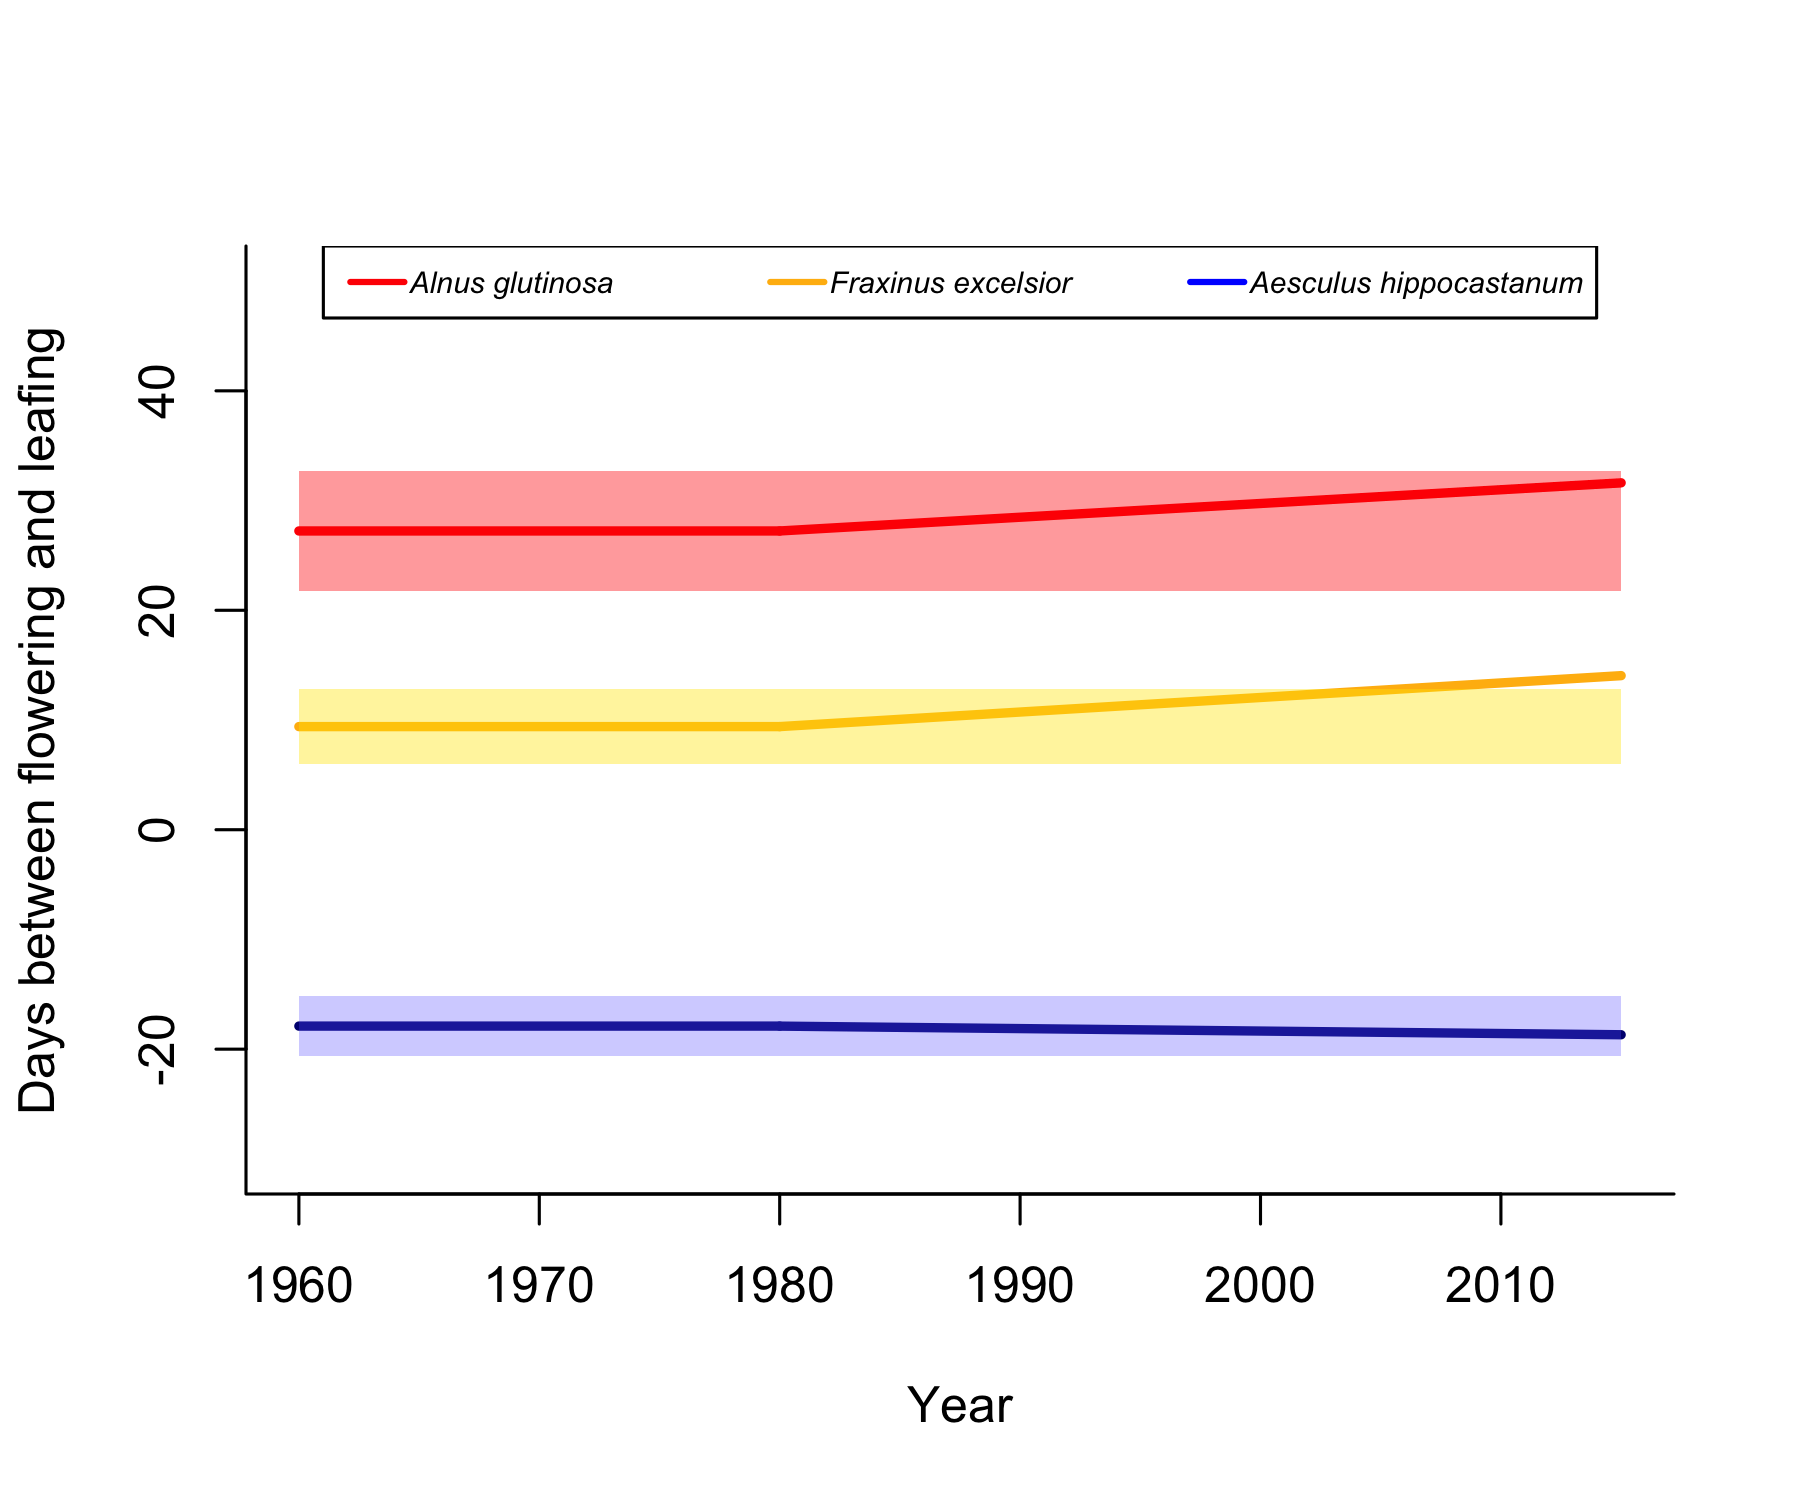
\includegraphics[width=.75\textwidth]{..//figure/FLS_climate_change.png}\\
\caption{Trends in average time between flowering and leafing across Europe for three tree species from 1960 to 2015. Highlighted regions indicate historic range of FLS variability. For all species, the time between flowering and leafing is increasing in step with climate change, but the rate of change differs between species and sites.}
    \label{fig:Figure 1}
    \end{figure}

\newpage
\noindent \emph{References mentioned in cover letter}
\begin{footnotesize}
\begin{enumerate}
\item Whitehead, D. 1969. Wind Pollination in the Angiosperms: Evolutionary and Environmental Considerations. \emph{Evolution},23: 28-35.
\item Reich, P.B. \& Borchert, R. 1984. Water-stress and tree phenology in a tropical dry forest in the lowlands of Costa-Rica. \emph{Journal of Ecology}, 72: 61-74.
\item Primack, R. B. 1987. Relationships Among Flowers, Fruits, and Seeds. \emph{Annual Review of Ecology and Systematics}, 18: 409-430.
\item Gougherty, A. V. \& Gougherty, S.W. 2018. Sequence of flower and leaf emergence in deciduous trees is linked to ecological traits, phylogenetics, and climate. \emph{New Phytologist}, 220: 121-131.
\item Bolmgren, K., et al. 2003. Contrasting flowering phenology and species richness in abiotically and biotically pollinated angiosperms. \emph{Evolution}, 57: 2001-2011.
\item Rathcke, B. \& Lacey, E. P. 1985. Phenological Patterns of Terrestrial Plants. \emph{Annual Review of Ecology and Systematics}, 16: 179-214.
\item Cleland, E.E., et al. 2007. Shifting plant phenology in response to global change. \emph{Trends in Ecology & Evolution}, 22: 357-365.
\end{enumerate}
\end{footnotesize}
\end{document}
